
\documentclass[12pt]{article}
%\documentclass[smallextended,numbook]{svjour3}

\usepackage[english]{babel}
\usepackage[utf8x]{inputenc}
\usepackage{pdfpages}
\usepackage{amsfonts,dsfont}
\usepackage{amsmath}
\usepackage{amssymb}
\usepackage{amsthm} %commenter pour style MP
\usepackage{bm}
\usepackage{natbib}
\usepackage{hyperref}
\usepackage{algorithm2e}
\usepackage{enumitem}
\usepackage[capitalise]{cleveref}
%\usepackage[capitalise,poorman]{cleveref}

\setlength {\marginparwidth }{2cm}
\usepackage{todonotes}
\usepackage[all]{xy} 

\makeatletter \let\cl@part\relax \makeatother

%\usepackage[top=1cm, bottom=1cm, left=1cm, right=1cm]{geometry}
\usepackage[top=2cm, bottom=2cm, left=2cm, right=2cm]{geometry}
\usepackage{xcolor}
\usepackage{tikz}
\usetikzlibrary{calc}
\usetikzlibrary{intersections}
\tikzset{offset/.style={to path={%
    -- ($(\tikztostart)!#1cm!(\tikztotarget)$)}},
         offset/.default=1}
\tikzset{>=latex}


\renewcommand{\thesection}{\Alph{section}}
\usepackage{pgfplots}

\newcommand{\mf}[1]{\begin{color}{brown}\texttt{MF:#1}\end{color}}

\newcommand{\TODO}{\begin{color}{red}TODO\end{color}}

\newcommand{\tco}{tCO_2eq}

\newcommand{\ques}[1]{\begin{enumerate}[resume]
\item  #1
\end{enumerate}}

\newcommand{\rep}[1]{\textit{Réponse :} #1 }
\renewcommand{\rep}[1]{ }

\usepackage{subcaption}
%\usepackage[colorinlistoftodos,bordercolor=orange,backgroundcolor=orange!20,linecolor=orange,textsize=scriptsize]{todonotes}


%% Theorems
\newtheorem{hypo}{Assumption}
\Crefname{hypo}{Assumption}{Assumptions}

\newtheorem{theorem}{Theorem}
\newtheorem{lemma}[theorem]{Lemma}
\newtheorem{remark}[theorem]{Remark}
\newtheorem{cor}[theorem]{Corollary}
\newtheorem{prop}[theorem]{Proposition}
\newtheorem{defi}[theorem]{Definition}
\newtheorem{conj}{Conjecture}
\newtheorem{nota}{Notation}
\theoremstyle{remark}
\newtheorem{exa}{Example}





\title{TD \\Modèle 
DICE (Dynamic Integrated Climate Economy) \\
de Nordhaus simplifié }

\author{Maël Forcier}


\begin{document}
\maketitle


\section{Modélisation économique}

Le modèle de Nordhaus est un modèle de macroéconomie qui étudie l'évolution de l'économie mondiale. Le modèle est dynamique, les variables non-constantes seront indicés par le temps $t$. La variable principale est le capital, noté $K_t$, c'est-à-dire la valeur en \$ de tous les biens matériels ou immatériels dans le monde. Le produit intérieur brut (PIB) en \$ noté $Q_t$ est la somme de tous les revenus annuels d'une économie. La consommation notée $C_t$ est la somme en \$ de tous les biens et services perissables utilisés pendant une année.L'investissement en \$ noté $I_t$ est l'ensemble des 

\begin{enumerate}
\item On suppose que le PIB n'est utilisé que pour la consommation et l'investissement. Proposer une équation reliant $Q_t$, $C_t$ et $I_t$.
\end{enumerate}
\rep{ $Q_{t}=C_t + I_t$ }
\begin{enumerate}[resume]
\item  Le capital accumulé se déprécie à un taux $\delta_K$ qui le fait diminuer entre chaque étape, mais l'investissement permet de générer du nouveau capital. Proposer une équation dite de dynamique reliant $K_{t}$, $K_{t-1}$, $I_t$ et $\delta_K$.
\end{enumerate}
\rep{ $K_{t}=(1-\delta_K)K_{t-1}+I_t$ }

L'équation de Cobb-Douglas, classique en macroéconomie pour étudier la croissance, fait l'hypothèse que le PIB $Q_t$ est égal au produit $AK_t^\gamma L_t^{1-\gamma}$ où $A$ est appelé le facteur de productivité, $\gamma$ l'élasticité du capital et $L_t$ le travail, souvent approximé comme égal à la population. Pour simplifier, nous négligerons l'effet de la population et prendrons une élasticité au capital de $\gamma=1$. Pour prendre en compte le réchauffement climatique, Nordhaus propose d'ajouter un autre facteur $\Omega_t$ qui combine les dégats causées par le réchauffement climatique et les coûts  de l'investissement pour le climat. 
\ques{  Proposer une équation de Cobb-Douglas simplifiée (sans le travail) et qui prend en compte le climat en reliant $Q_{t}$, $A$,$\Omega_t$ et $K_{t}$.
}
\rep{ $Q_{t}=A \Omega_t K_t$}
Selon Eurostat, l'investissement représente environ de 23 \% en Europe et cette part est stable entre 2005 et 2009. Pour simplifier, on considèrera que l'investissement représente un quart du PIB : $I_t=Q_t/4$.
\ques{Avec cette hypothèses, simplifier les équations pour obtenir une relation entre $K_t$, $K_{t-1}$, $A$, $\Omega_t$ et $\delta_K$}
\rep{\begin{equation*} K_t=\frac{1- \delta_K}{1- \frac{A\Omega_t}{4}} \end{equation*}}


\section{Modélisation de l'effet du climat}

Nous allons maintenant modéliser les dégâts causées par le réchauffement climatique. Nordhaus choisit de de modéliser $\Omega_t$ comme le rapport d'un accroissement du à un taux $TC_t$ modélisant les coûts d'investissement dans les technologies bas carbone et à une dépréciation du à un taux $d_t$ modélisant les dommages que le réchauffement climatique cause sur le PIB :
\begin{equation*}
\Omega_t=\frac{1-TC_t}{1+d_t}
\end{equation*}
On note $T_t$ l'augmentation de la température en °C par rapport à l'ère préindustrielle (pour simplifier on fera l'hypothèse qu'elle est égale à la température moyenne en 2000). En s'appuyant sur quelques papiers économiques de son époque, Nordhaus fait l'hypothèse qu'un réchauffement climatique de 3°C fait baisser le PIB de 1,33 \%. Constatant que les dégats sur le PIB ne sont pas linéaires avec la température, Nordhaus fait l'hypothèse que les dégâts évoluent comme une fonction au carré de la température. On suppose également que si la température n'augmente pas, on n'observe pas de dégât.

\ques{  Avec ces hypothèses, proposer une relation entre $d_t$ et $T_t$.
}
\rep{ \begin{equation*}
d_{t}=0,0133(\frac{T_t}{3})^2 \end{equation*}
}

On veut maintenant modéliser l'effet des émissions de gaz à effet de serre sur la température. On note $M_t$ le total d'émissions cumulées dans l'atmosphère en $G\tco$. Pour rappel, le GIEC présente dans le graphique ci-dessous le lien entre les émissions cumulées et l'augmentation de la Température.
\begin{figure}[h]
\centering
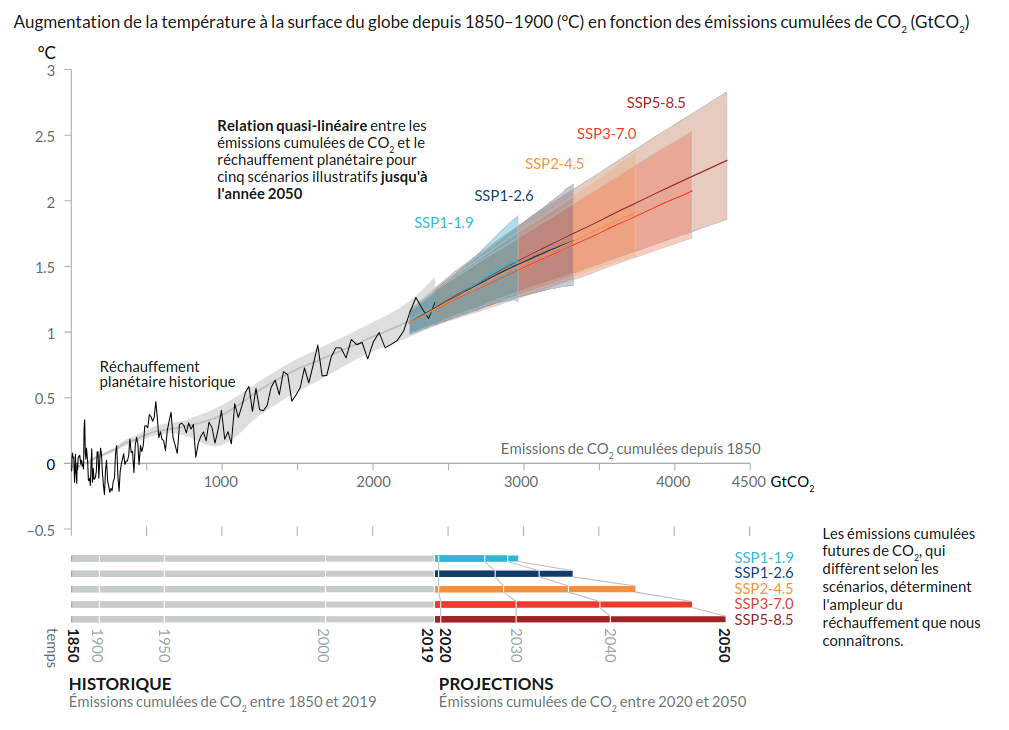
\includegraphics[scale=0.5]{images/Lien_GES_Temperature.png}
\end{figure}


\ques{A partir du graphique ci-dessous, proposer une relation simple entre $T_t$ et $M_t$}
\rep{\begin{equation*} T_t= \frac{M_t}{2000}\end{equation*}}

On note $E_t$ les emissions à chaque pas de temps (flux), là où $M_t$ constitue le stock.
Les émissions évoluent selon une dynamique particulière entre les océans, l'atmosphère et le rayonnement solaire, qui suit les équations de la thermodynamique et de la mécanique des fluides.
Pour simplifier, on considérera que toutes les émissions restent dans l'atmosphère.
\ques{ Avec ces hypothèses simplifiées, proposer une équation entre $M_t$, $M_{t-1}$ et $E_t$.}
\rep{$M_t =M_{t-1} +E_t$}

Enfin, Nordhaus considère une variable $\mu_t$ appelé "taux de contrôle des émissions".
Elle modélise l'effort des gouvernements pour contrôler les émissions de l'économie mondiale :
\begin{equation*}
E_t=(1-\mu_t)\sigma Q_t
\end{equation*}
Avec $\sigma$ une constante qui représente le facteur d'émission du PIB dans un scénario sans contrôle $\mu_t=0$. Dans le cas $\mu_t=1$, le contrôle est total, on émet pas de gaz à effet de serre.
\ques{Exprimer $T_t$ en fonction de $\sigma$, $\mu_1, \cdots, \mu_t$ et $Q_1, \cdots ,Q_t$}.
\rep{\begin{equation*}T_t= \frac{\sigma}{2000} \sum_{k=1}^t (1-\mu_k) Q_k  \end{equation*}}

\section{Scénario contrôle total}


\section{Scénario sans contrôle}


\section{Discussion et critiques}
\begin{enumerate}[resume]
\item Quelles variables sont endogènes, exogènes ?
\item Comment qualifier le modèle top-down/bottom-up, statique/dynamique, stochastique/déterministe, d'optimisation, discret/continu ?
\item Quelles hypothèses pourraient être ajoutées ?
\end{enumerate}

\section{Comparaison avec le papier d'origine}
\begin{enumerate}[resume]
\item Quelles sont les simplifications que l'on a faite par rapport au modèle DICE du papier de Nordhaus de 1992 ?
\end{enumerate}


\end{document}